\documentclass[12pt,a4paper,titlepage,headinclude,bibtotoc]{scrartcl}

%---- Allgemeine Layout Einstellungen ------------------------------------------

% Für Kopf und Fußzeilen, siehe auch KOMA-Skript Doku
\usepackage[komastyle]{scrpage2}
\pagestyle{plain}
\setheadsepline{0.5pt}[\color{black}]
\automark[section]{chapter}


%Einstellungen für Figuren- und Tabellenbeschriftungen
\setkomafont{captionlabel}{\sffamily\bfseries}
\setcapindent{0em}


%---- Weitere Pakete -----------------------------------------------------------
% Die Pakete sind alle in der TeX Live Distribution enthalten. Wichtige Adressen
% www.ctan.org, www.dante.de

% Sprachunterstützung
\usepackage[ngerman]{babel}

% Benutzung von Umlauten direkt im Text
% entweder "latin1" oder "utf8"
\usepackage[utf8]{inputenc}

% Pakete mit Mathesymbolen und zur Beseitigung von Schwächen der Mathe-Umgebung
\usepackage{latexsym,exscale,stmaryrd,amssymb,amsmath}


\usepackage[nointegrals]{wasysym}
\usepackage{eurosym}

% Anderes Literaturverzeichnisformat
%\usepackage[square,sort&compress]{natbib}
\usepackage{hyperref}
% Für Farbe
\usepackage{color}
\usepackage{graphicx}
\usepackage{wrapfig}
\usepackage{subfigure}

% Caption neben Abbildung
\usepackage{sidecap}


% Befehl für "Entspricht"-Zeichen
\newcommand{\corresponds}{\ensuremath{\mathrel{\widehat{=}}}}
% Befehl für Errorfunction
\newcommand{\erf}[1]{\text{ erf}\ensuremath{\left( #1 \right)}}


%Fußnoten zwingend auf diese Seite setzen
\interfootnotelinepenalty=1000

%Für chemische Formeln (von www.dante.de)
%% Anpassung an LaTeX(2e) von Bernd Raichle
\makeatletter
\DeclareRobustCommand{\chemical}[1]{%
  {\(\m@th
   \edef\resetfontdimens{\noexpand\)%
       \fontdimen16\textfont2=\the\fontdimen16\textfont2
       \fontdimen17\textfont2=\the\fontdimen17\textfont2\relax}%
   \fontdimen16\textfont2=2.7pt \fontdimen17\textfont2=2.7pt
   \mathrm{#1}%
   \resetfontdimens}}
\makeatother
\usepackage{textcomp}
\usepackage{upgreek}
%\begin{document}
%$\upmu$
%\end{document}
%Honecker-Kasten mit $$\shadowbox{$xxxx$}$$
\usepackage{fancybox}

%SI-Package
\usepackage{siunitx}

%keine Einrückung, wenn Latex doppelte Leerzeile
\parindent0pt

%Bibliography \bibliography{literatur} und \cite{gerthsen}
%\usepackage{cite}
\usepackage{babelbib}
\selectbiblanguage{ngerman}

\usepackage{siunitx}
%\begin{document}
 % \SI{1.55}{\micro\metre}
\sisetup{math-micro=\text{µ},text-micro=µ}
\usepackage{amsmath}
\begin{document}

\begin{titlepage}
\centering
\textsc{\Large Physikalisch- Chemisches Grundpraktikum\\[1.5ex] Universität Göttingen}

\vspace*{0.5cm}

\rule{\textwidth}{1pt}\\[0.5cm]
{\huge \bfseries
  Versuch 12: \\[1.5ex]
  Joule-Thomson-Effekt}\\[0.5cm]
\rule{\textwidth}{1pt}

\vspace*{0.5cm}


\begin{Large}
\begin{tabular}{ll}
Durchführende: &  Isaac Maksso, Julia Stachowiak\\
Assistentin: & Katharina Meyer \\
 Versuchsdatum: & 27.10.2016\\
 Datum der ersten Abgabe: & 03.11.2017\\
\end{tabular}
\end{Large}

\vspace*{0.5cm}

\begin{Large}
\fbox{
  \begin{minipage}[t][8cm][t]{8cm}
  
 TestGithub\\ 
 Messwerte:\\
  Literaturwerte:\\
  $M_\mathrm{Campher} = 152,23 \mathrm{g{~} mol^{-1}}\protect\footnotemark 
  $\\
  $M_\mathrm{KCl} = 74,55 \mathrm{g{~} mol^{-1}} \protect\footnotemark 
$\\\\
  
  \end{minipage}
}
\end{Large}
\footnotetext{Quelle: https://de.wikipedia.org/wiki/Campher, aufgerufen am 31.12.16}
 \footnotetext{Quelle: http://www.chemie.de/lexikon/Kaliumchlorid.html, aufgerufen am 31.12.16}
\end{titlepage}


\tableofcontents

\newpage


\section{Experimenteller Aufbau}


\begin{figure} [h!]
\begin{center}
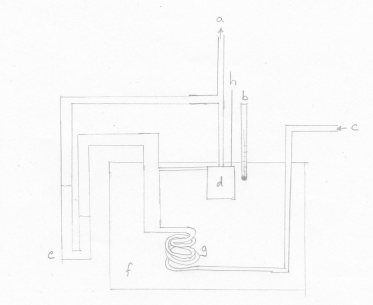
\includegraphics[scale=1.5]{VersuchsaufbauJT.png} \end{center}
\caption{Versuchsaufbau.}
\end{figure}

a) Gasanschluss\\
b)Thermometer\\
c)Gaseinlass\\
d)Drosselstelle\\
e)Differenzdruckmanometer\\
f)Wärmebad\\
g)Wärmetauscher\\
h)$\Delta$T-Messstelle\\

 
 


\section{Auswertung}

%Darstellung und Auswertung der Messergebnisse
%Fehlerrechnung und Fehlerdiskussion (statistische und systematische fehler)
%Abschätzung systematischer Fehler
%Endergebnis mit Fehlerangabe


\subsection{Berechnung des mitteleren Joule-Thomson-Koeffizienten}
Der mittlere Joule-Thompson-Koeffizient entspricht der Steigung bei einer Auftragung von $\Delta$ T gegen $\Delta$ p. Hierbei wird der Differentialquotient durch einen Differenzenquotienten ersetzt. Der Fehler ergibt sich als der Fehler der Auftragung.\\

\begin{equation}
T_1 - T_2 = <\mu_{JT}> \cdot (p_1 - p_2)
\end{equation}

Die sich ergebenden Steigungen sind in nachfolgender Tabelle aufgelistet. Die Fehler wurden als Standardfehler der Auftragung berechnet. Die einzelnen Auftragungen sind im Anhang zu finden.\\

\begin{table} [h]
\begin{tabular} {l | c|  c | c}
	 &  T [K] & $<\mu_{JT}>$ [$  10^{-5}\cdot \frac{\mathrm{K}}{\mathrm{bar}}$] & $\Delta <\mu_{JT}>$  [$  10^{-7}\cdot \frac{\mathrm{K}}{\mathrm{bar}}$]\\
	 \hline
	  $CO_\mathrm{2}$ & 273,25 & 1,20 & 3,80 \\
	   & 295,95 & 1,01 & 5,97\\
	  & 323,95 & 0,710 & 4,67\\
	\hline
	$N_\mathrm{2}$ & 273,25 & 0,181  &  2,20\\
	& 295,95 & 0,175 & 2,35\\
	& 323,95& 0,120& 1,30\\
\end{tabular}
\end{table}


\subsection{Herleitung $c_\mathrm{v}^\mathrm{ vib}$}

Zur Berechnung von $\mu_{JT}$ wird neben tabellierten Größen vor allem die molare Wärmekapazität bei konstantem Druck $c_\mathrm{p}$ benötigt. Diese wiederum ergibt sich aus der molaren Wärmekapazität bei konstantem Volumen $c_\mathrm{v}$:

\begin{equation}
c_\mathrm{p} = c_\mathrm{v} +R
\end{equation}

Da Wärme in Form von Schwingungsenergie(Vibration), Rotationsenergie und Bewegungsenergie(Translation) von einzelnen Molekülen aufgenommen und somit gespeichert werden kann, liefern diese je ihren Beitrag zur molaren Wärmekapazität(die Energieaufnahme in Form von Elektronenanregung spielt in diesem Fall keine Rolle und wird daher vernachlässigt):

\begin{equation}
c_\mathrm{v} = c_\mathrm{v}^\mathrm{ vib} + c_\mathrm{v}^\mathrm{ rot} + c_\mathrm{v}^\mathrm{trans}  
\end{equation}

Die einzelnen Beiträge ergeben sich je aus den Freiheitsgraden für Moleküle. Die sind je nach Atomzahl und Geometrie (linear/gewinkelt) unterschiedlich. $N_2$ und $CO_2$ sind beide linear und haben daher ähnliche Werte:\\


\begin{table} [h]
\begin{tabular} {l | c|  c | c}
	 & $c_\mathrm{v}^\mathrm{ vib}$  & $c_\mathrm{v}^\mathrm{ rot}$ & $c_\mathrm{v}^\mathrm{trans}$\\
	 \hline
	 $N_2$ & $k_B$T & $k_B$T &$\frac{3}{2}k_B$T\\
	  $CO_2$ & 4$k_B$T & $k_B$T &$\frac{3}{2}k_B$T\\
\end{tabular}
\end{table}

Da die Schwingung erst bei sehr hohen Temperaturen vollständig angeregt ist, muss folgende Formel verwedet werden, die hier hergeleitet wird: \\


\begin{equation}
c_\mathrm{v}^\mathrm{ vib} = R\cdot(hv\beta)^2 \frac{\mathrm{exp}(hv\beta)}{\mathrm{exp}(hv\beta -1)^2}
\end{equation}


mit $\beta=\frac{1}{k_{B} \cdot T}$.\\

Grundlage bildet die Vibrationszustandssumme des Systems:\\

\begin{equation}
Z_{vib}= \left[\frac{\mathrm{exp}(-\frac{hv}{2k_BT})}{1-\mathrm{exp}(-\frac{hv}{k_BT})}\right]^N
\end{equation}

Bei adiabatischer Prozessführung ist die Wärmezufuhr/-abgabe gleich der Änderung der inneren Energie. Die Vibrationszustandssumme steht mit letzterer folgendermaßen im Zusammenhang:\\

\begin{equation}
U_{vib}= -k_BT^2 \frac{\partial lnZ_{vib}}{\partial T} = N\frac{hv}{2} +\frac{Nhv}{exp\left(\frac{hv}{k_BT}\right)-1}= U_\mathrm{m}^\mathrm{vib} = R \Theta \left[ \frac{1}{2} + \frac{1}{\mathrm{exp}(\frac{\Theta_\mathrm{vib}}{T} -1)}\right]
\end{equation}

Mit\\

\begin{equation}
\Theta_\mathrm{vib} = \frac{hv}{k_\mathrm{B}}
\end{equation}


Die Ableitung der molaren inneren Energie ergibt die molare Wärmekapazität:\\


\begin{equation}
c_\mathrm{v} = \frac{\partial U_\mathrm{m}}{\partial T}\bigg \vert_\mathrm{V}
\end{equation}

Analog gilt:

\begin{equation}
c_\mathrm{v}^\mathrm{vib} = \frac{\delta U_\mathrm{m}^\mathrm{vib}}{\delta T}\bigg \vert_\mathrm{V}
\end{equation}

Das ganze abgeleitet ergibt wiederum $c_v^{vib}$ als herzuleitende Formel.\\


\subsection{Berechnung von $\mu_{JT}$ aus der Virialgleichung}

Der Unterschied eines realen Gases zum idealen Gas wird mittels Virialentwicklung beschrieben, wobei hier ein Abbruch nach dem 2. Virialkoeffizienten stattfindet.\\

\begin{equation}
pV_\mathrm{m} = RT + B(T) \cdot p
\end{equation}

Wie in obiger Gleichung gut zu sehen ist, bildet der 2. Virialkoeffizient einen Korrekturterm für den Druck im Bezug zum idealen Gasgesetz, der linear vom Druck abhängig ist.
Der Joule-Thomson-Koeffizient kann in Abhängigkeit des 2. Virialkoeffizienten folgendermaßen ausgedrückt werden:

\begin{equation}
\mu_{JT} = \frac{1}{c_\mathrm{p}}\left( T \frac{\delta B}{\delta T} \bigg \vert_\mathrm{p} - B\right)
\end{equation}

Hier wird mit der reduzierten Temperatur gerechnet. dh.: 

\begin{equation}
T^* = \frac{T}{\varepsilon}
\end{equation}

$\varepsilon$ ist hierbei eine Stoffkonstante der Einheit Kelvin, die für $N_\mathrm{2}$ und $CO_\mathrm{2}$ unterschiedliche Werte annimmt. Somit ist die redizierte Temperatur eine dimensionslose Größe, mit der sich leichter rechnen lässt.\\ 
Somit wird $\mu_{JT}$ letzendlich folgendermaßen berechnet:\\

\begin{equation}
\mu_{JT} = \frac{1}{c_\mathrm{p}}\left( T^* \frac{\partial B^*(T^*)}{\partial T^*} \bigg \vert_\mathrm{p} - B^*(T^*)\right)
\end{equation}

Die Werte für $B^*(T^*)$ und $\mathrm{T^*}\frac{\mathrm{dB^*(T^*)}}{\mathrm{dT^*}}$ pro $T^*$ wurden einer Tabelle am Ende des Praktikumsskriptes entnommen.\protect\footnote{Hirschfelder, Curtiss, Bird, New Yorck 1954}

Folgende Größen ergeben sich:\\

\begin{table} [h]
\begin{tabular} {l | c|  c | c}
	 &  T [K] &  $c_\mathrm{p}$ [$\frac{\mathrm{J}}{\mathrm{K}\cdot \mathrm{mol}}$] & $ <\mu_{JT}>$ [$\frac{\mathrm{K}}{\mathrm{bar}}$] \\
	 \hline
	  $N_\mathrm{2}$ & 273,25 & 37,4150658304 &  \\
	   & 295,95 & 37,4150636569 & \\
	  & 323,95 & 37,4150806757 & \\
	\hline
	$CO_\mathrm{2}$ & 273,25& 37,4150756767  &  \\
	& 295,95 & 37,4150687407 & \\
	& 323,95& 37,4150583339& \\
\end{tabular}
\end{table}



%$\frac{\partial B^*}{\partial T^*}= -0,241$ Außerdem gilt die Beziehung:\\

%\begin{equation}
%B(T) = b_\mathrm{0}B^*(T^*) = b_0(0,904 -0,241T^*)
%\end{equation}

%Mit $b_0= \frac{2}{3}\pi N_\mathrm{L} \sigma^3$ und  lässt sich somit der Joule- Thompson- Koeffizient aus der Wärmekapazität bei konstantem Druck errechnen:\\

%\begin{equation}
%\mu_{JT} = \frac{1}{c_\mathrm{p}} \left(T\left(-0,241b_0\right) - b_0\left(0,904-0,241T^*\right)\right)
%\end{equation}

%Letzendlich wurden die $\mu_{JT}$-Koeffizienten mit folgender Formel ermittelt:\\

%\begin{equation}
%\frac{1}{\mathrm{c_p}}\left(T^*\frac{dB^*(T^*)}{dT^*} -B^*(T^*)\right)
%\end{equation}

\subsection{Fehlerrechnung}
Nach der Gauß'schen Fehlerfortpflanzung

\begin{equation}
\Delta f = \sqrt{\sum_\mathrm{i} \left(\frac{d}{dx_\mathrm{i}}\right)^{2} \cdot \Delta x_\mathrm{i}^2}
\end{equation}


ergibt sich für $\mu_{JT}$ folgender Fehler:\\








\subsection{Vergleich mit den Literaturwerten}
%Für die Molmasse der Substanz im Cyclohexan ergeben sich folgende Werte:\\
%$M_A = (13 \cdot 10 \pm 3 \cdot 10){~} \mathrm{g{~}mol^{-1}}$\\\\
%$M_B = (12 \cdot 10 \pm 2 \cdot 10){~} \mathrm{g{~}mol^{-1}}$\\\\
%Dabei handelt es sich um Campher, dieses hat eine Molmasse von $ 152,23{~} \mathrm{g{~}mol^{-1}}$ \footnote{https://de.wikipedia.org/wiki/Campher abgerufen am \textbf{13.12.2015}} Beide Werte weichen um $15-21\%$ nach unten hin ab, dies legt einen systematischen Fehler nahe, wobei der Wert 1 noch im Fehlerintervall liegt.\\\\
%Für die Molmasse der im Wasser gelösten Substanz ergibt sich:\\\\
%$M_A = (6 \cdot 10 \pm 3 \cdot 10){~} \mathrm{g{~}mol^{-1}}$\\\\
%$M_B = (5\cdot 10 \pm 3\cdot 10 ){~} \mathrm{g{~}mol^{-1}}$\\\\
%Es handelt sich bei der im Wasser gelösten Substanz um Kaliumchlorid, dieses hat eine Molmasse von $74,55{~} \mathrm{g{~}mol^{-1}}$ {~}\footnote{https://de.wikipedia.org/wiki/Kaliumchlorid abgerufen am \textbf{09.12.2015}} Die starke Abweichung von $20-30\%$ der Werte lässt sich nicht mithilfe der Fehlerfortpflanzung erklären, daher muss es sich um systematische Fehler handeln. 



\section{Diskussion}
Diskussion vom Endergebnis und seiner Genauigkeit
Vergelich mit Literaturwerten
kritische Analyse des Experiments




\section{Anhang}
 














\newpage


\subsection{Literaturverzeichnis}
1\quad Eckhold, Götz: \emph{Praktikum I zur Physikalischen Chemie}, Institut für Physikalische Chemie, Uni Göttingen, \textbf{2014}.

\vspace{0,5 cm}

2 \quad Eckhold, Götz: \emph{Statistische Thermodynamik}, Institut für Physikalische Chemie, Uni Göttingen, \textbf{2012}.

\vspace{0,5cm}

3 \quad Eckhold, Götz: \emph{Chemisches Gleichgewicht}, Institut für Physikalische Chemie, Uni Göttingen, \textbf{2015}.\\

\end{document}


